\documentclass[conference]{IEEEtran}

% --- PACKAGES ---
\usepackage[T1]{fontenc}
\usepackage{lmodern}
\usepackage{graphicx}       % For including images
\usepackage{amsmath}        % For advanced math
\usepackage{amssymb}        % For math symbols
\usepackage{booktabs}       % For professional tables
\usepackage{url}            % For formatting URLs
\usepackage{cite}           % For IEEE-style citations
\usepackage{verbatim}       % For code-like text
\usepackage[scaled=0.9]{helvet} % For sans-serif text (e.g., UI elements)
\usepackage{caption}        % Better caption control

\graphicspath{{figures/}}   % Figures folder

% --- DOCUMENT START ---
\begin{document}

% --- TITLE AND AUTHOR ---
\title{Multi-Modal Predictors for Cardiovascular Disease Risk and Outcomes:\\
Deliverable 2 -- Implementation and Early Evaluation}

% For a course paper, a compact block reads well and is acceptable.
\author{
    \IEEEauthorblockN{Angel Morenu}
    \IEEEauthorblockA{
        University of Florida\\
        EEE 6778 -- Applied Machine Learning II (Fall 2025)\\
        Instructor: Dr. Ramirez-Salgado\\
        Email: angel.morenu@ufl.edu
    }
}

% Creates the title
\maketitle

% --- ABSTRACT ---
\begin{abstract}
Cardiovascular disease (CVD) remains the leading cause of mortality worldwide, motivating early and reliable risk assessment tools. This work implements a multi-modal predictive framework that fuses demographic/clinical tabular data, hospital admissions records, and physiological electrocardiogram (ECG) signals to estimate CVD risk. The pipeline combines robust preprocessing and baselines in scikit-learn with a PyTorch 1D convolutional model for ECG feature extraction and a fusion classifier. An interactive Streamlit interface enables local, privacy-preserving inference and ECG visualization. I report a fully functional end-to-end system---data ingestion, preprocessing, training, evaluation, and user interaction---with preliminary held-out performance (Accuracy 0.476, ROC AUC 0.427, PR AUC 0.539, Brier 0.325). Although early metrics are modest, results confirm stable training and validate the feasibility of multi-modal fusion for CVD risk modeling. I outline key challenges (class imbalance, ECG normalization, calibration) and next steps (class-weighted loss, early stopping, SHAP-based interpretability, and edge deployment).
\end{abstract}

% --- SECTIONS ---

\section{Introduction and Motivation}
Cardiovascular disease (CVD) remains the leading cause of morbidity and mortality globally, imposing significant burdens on public health systems and economies \cite{goodfellow2016deep}. Early and accurate identification of at-risk individuals is central to prevention and intervention. Classical risk models (e.g., Framingham) rely on limited, unimodal features (age, blood pressure, lipids, smoking), which can under-represent the complexity of cardiovascular pathophysiology and the richness of modern physiological sensing.

I address this gap with a multi-modal predictive framework that integrates heterogeneous sources:
\begin{itemize}
    \item \textbf{Demographic/Clinical Data:} structured (tabular) risk indicators (age, blood pressure, cholesterol, lifestyle).
    \item \textbf{Hospital Admissions:} categorical context from encounter metadata (admission type, diagnosis codes).
    \item \textbf{Physiological Signals:} 1D ECG waveforms that capture transient electrical activity.
\end{itemize}
I hypothesize that complementary modalities provide an additive signal for discrimination and robustness. I implement scikit-learn preprocessing \cite{pedregosa2011scikit} and PyTorch-based deep learning \cite{goodfellow2016deep} to extract ECG features via a lightweight 1D-CNN and fuse them with tabular embeddings. Since Deliverable~1, the system moved from concept to a reproducible prototype with end-to-end training, evaluation, and an interactive Streamlit demo. This report documents implementation and early results, establishing a baseline for optimization and interpretability.

% --- Figure 1: two-column architecture (prioritize figures/multimodal_cvd_architecture.png) ---
\begin{figure*}[!t]
    \centering
    % Prioritize the requested path (figures/multimodal_cvd_architecture.png), then fall back to other locations/formats.
    \IfFileExists{\detokenize{figures/multimodal_cvd_architecture.png}}{%
        \includegraphics[width=0.92\textwidth]{\detokenize{figures/multimodal_cvd_architecture.png}}%
    }{%
        \IfFileExists{\detokenize{figures/multimodal_cvd_architecture.pdf}}{%
            \includegraphics[width=0.92\textwidth]{\detokenize{figures/multimodal_cvd_architecture.pdf}}%
        }{%
            \IfFileExists{\detokenize{ui/multimodal_cvd_architecture.png}}{%
                \includegraphics[width=0.92\textwidth]{\detokenize{ui/multimodal_cvd_architecture.png}}%
            }{%
                \IfFileExists{\detokenize{ui/multimodal_cvd_architecture.pdf}}{%
                    \includegraphics[width=0.92\textwidth]{\detokenize{ui/multimodal_cvd_architecture.pdf}}%
                }{%
                    \IfFileExists{\detokenize{multimodal_cvd_architecture.png}}{%
                        \includegraphics[width=0.92\textwidth]{\detokenize{multimodal_cvd_architecture.png}}%
                    }{%
                        \IfFileExists{\detokenize{multimodal_cvd_architecture.pdf}}{%
                            \includegraphics[width=0.92\textwidth]{\detokenize{multimodal_cvd_architecture.pdf}}%
                        }{%
                            \fbox{%
                                \parbox[b][5cm][c]{0.92\textwidth}{\centering Architecture figure not found\\(expected: figures/multimodal\_cvd\_architecture.png).}%
                            }%
                        }%
                    }%
                }%
            }%
        }%
    }
    \caption{
        \textbf{System Architecture of the Multi-Modal CVD Risk Predictor.}
        The pipeline integrates three heterogeneous data sources---tabular demographic data, hospital admission records, and ECG waveforms---processed through scikit-learn and PyTorch modules.
        The architecture consists of: (1) preprocessing and feature scaling via \texttt{ColumnTransformer}, (2) per-modality modeling with classical baselines and neural encoders, (3) fusion and classification through dense layers, and (4) outputs delivered through the Streamlit interface and conceptual Edge-AI deployment (e.g., smartwatch scenario).
    }
    \label{fig:architecture}
\end{figure*}

\section{System Architecture and Pipeline}
The architecture (Fig.~\ref{fig:architecture}) is modular and reproducible, transforming raw multi-source data into actionable risk estimates:
\begin{enumerate}
    \item \textbf{Data Ingestion and Preprocessing (scikit-learn).} Tabular features (demographics, vitals, lifestyle) are imputed (median for continuous; mode for categorical), one-hot encoded, and scaled with \texttt{StandardScaler}. ECG sequences are trimmed/padded to 2{,}000 samples and per-signal normalized to zero mean/unit variance.
    \item \textbf{Baseline Models.} Classical baselines (logistic regression, random forest) are implemented for tabular data using scikit-learn \cite{pedregosa2011scikit,raschka2022python} to establish reference performance.
    \item \textbf{Feature Alignment.} Processed arrays are saved under \texttt{data/processed/} with a manifest mapping each \texttt{patient\_id} across modalities, ensuring consistent indexing in batches.
    \item \textbf{Model Training (PyTorch).} I support an ECG-only regime (Week~4 sanity check) and a fused regime (Week~5) combining tabular and ECG embeddings into a binary classifier.
    \item \textbf{Evaluation.} Accuracy, ROC AUC, PR AUC, and Brier score are computed on a held-out test set; confusion matrices and curves are exported to \texttt{results/}.
    \item \textbf{Interface.} A Streamlit app loads the checkpoint and transformer for interactive predictions and plots the ECG waveform.
    \item \textbf{Datasets \& Preprocessing.}
        \begin{table}[!t]
        \renewcommand{\arraystretch}{1.15}
        \caption{Datasets and Preprocessing Summary}
        \label{tab:data}
        \centering
        \begin{tabular}{@{}p{2.3cm}p{2.8cm}p{2.8cm}@{}}
        \toprule
        \textbf{Modality} & \textbf{Source / Shape} & \textbf{Preprocessing} \\
        \midrule
        Tabular (risk factors) & Kaggle CVD; $(N\times D)$ features & Missing imputation (median/mode), one-hot encoding, \texttt{StandardScaler} \\
        Hospital admissions & Kaggle hospital; categorical codes & Cleaning, categorical encoding, time-alignment to tabular IDs \\
        ECG (1D) & PTB-XL (reformatted); $(1\times 2000)$ & Trim/pad to 2000, per-signal z-normalization; optional band-pass (planned) \\
        \bottomrule
        \end{tabular}
        \end{table}
\end{enumerate}

\section{Model Implementation Details}
\subsection{Tabular Encoder (MLP)}
Tabular inputs pass through two fully connected layers with ReLU and dropout ($p{=}0.3$), producing a 32-D embedding. This branch captures non-linear relationships among age, blood pressure, cholesterol, and lifestyle attributes.

\subsection{ECG Feature Extractor (1D-CNN)}
The ECG branch uses three convolutional blocks (kernel sizes 5,5,3; stride 2), each followed by batch normalization and ReLU, then global average pooling yields a 128-D embedding. This compact design balances expressiveness and efficiency for potential edge deployment.

\subsection{Fusion and Classifier}
The 160-D concatenated embedding (32-D tabular + 128-D ECG) is fed into a linear classifier producing logits for two classes (risk present/absent). Cross-entropy loss is used; class weights can mitigate imbalance.

\subsection{Training Setup and Reproducibility}
Training uses AdamW (learning rate $1\times10^{-3}$), batch size 64, for 10 epochs. Deterministic seeds are set across NumPy and Torch. Best checkpoints are saved to \texttt{artifacts/}. Experiments ran on macOS with PyTorch MPS acceleration. Code is organized under \texttt{src/} (model/train/eval) and \texttt{ui/} (Streamlit).

\begin{figure}[!t]
    \centering
    % Prefer canonical filenames (e.g., figures/confusion_matrix.png). If your file is
    % a macOS artifact like "._confusion_matrix.png", rename it to "confusion_matrix.png".
    \IfFileExists{\detokenize{figures/confusion_matrix.pdf}}{%
        \includegraphics[width=0.92\columnwidth]{\detokenize{figures/confusion_matrix.pdf}}%
    }{%
        \IfFileExists{\detokenize{figures/confusion_matrix.png}}{%
            \includegraphics[width=0.92\columnwidth]{\detokenize{figures/confusion_matrix.png}}%
        }{%
            \IfFileExists{\detokenize{figures/._confusion_matrix.png}}{%
                % fallback to the problematic macOS artifact if present
                \includegraphics[width=0.92\columnwidth]{\detokenize{figures/._confusion_matrix.png}}%
            }{%
                \fbox{%
                    \parbox[b][5cm][c]{0.92\columnwidth}{\centering Confusion matrix image not found\\(expected: figures/confusion\_matrix.pdf or .png)}%
                }%
            }%
        }%
    }
    \caption{Confusion Matrix (confusion\_matrix.png) on the held-out test set.}
    \label{fig:cm}
\end{figure}

\begin{table}[!t]
\renewcommand{\arraystretch}{1.15}
\caption{Training and Evaluation Setup}
\label{tab:train}
\centering
\begin{tabular}{@{}p{3.2cm}p{4.7cm}@{}}
\toprule
\textbf{Item} & \textbf{Setting} \\
\midrule
Optimizer / LR & AdamW, $1\times 10^{-3}$ \\
Batch size / Epochs & 64 / 10 \\
Loss & Cross-entropy (class-weighting planned) \\
Splits & 70/15/15 (stratified) train/val/test \\
Hardware & macOS (M1 Pro), PyTorch MPS \\
Metrics & Accuracy, ROC AUC, PR AUC, Brier; confusion matrix \\
Artifacts & \texttt{artifacts/best\_model.pt}, figures in \texttt{results/} \\
\bottomrule
\end{tabular}
\end{table}

\section{Interface Prototype}
The Streamlit app (\texttt{ui/MultiModalCVD\_app.py}) accepts structured inputs (sliders/dropdowns) and ECG upload (\texttt{.csv}/\texttt{.npy}). On \textit{Predict}, it preprocesses inputs, performs inference, and displays a calibrated probability with color-coded guidance (low/moderate/high risk). A waveform panel visualizes the ECG and reports key shape/length diagnostics. The app runs locally for privacy; a demo mode provides deterministic outputs if checkpoints are absent.

\begin{figure}[!t]
    \centering
    % Try the canonical names first, then fall back to the macOS dot-underscore artifact if present.
    \IfFileExists{\detokenize{figures/ui_demo.pdf}}{%
        \includegraphics[width=0.92\columnwidth]{\detokenize{figures/ui_demo.pdf}}%
    }{%
        \IfFileExists{\detokenize{figures/ui_demo.png}}{%
            \includegraphics[width=0.92\columnwidth]{\detokenize{figures/ui_demo.png}}%
        }{%
            \IfFileExists{\detokenize{figures/._ui_demo.png}}{%
                % macOS may create "._" resource-fork files; use it as a last-resort fallback
                \includegraphics[width=0.92\columnwidth]{\detokenize{figures/._ui_demo.png}}%
            }{%
                \fbox{%
                    \parbox[b][5cm][c]{0.92\columnwidth}{\centering UI demo image not found\\(expected: figures/ui\_demo.pdf or figures/ui\_demo.png).\\If you see a file named "._ui\_demo.png", consider renaming it to "ui\_demo.png".}%
                }%
            }%
        }%
    }
    \caption{
        \textbf{Streamlit Interface Prototype.}
        The interactive demo allows users to enter tabular inputs (e.g., age, BMI, blood pressure, cholesterol, smoker status, sex) and upload an ECG file in \texttt{.csv} or \texttt{.npy} format.
        The application normalizes inputs, performs model inference, and visualizes the waveform and predicted cardiovascular risk probability with interpretive guidance (e.g., low, moderate, or high risk). 
        All processing occurs locally to preserve user privacy.
    }
    \label{fig:ui_demo}
\end{figure}

\section{Early Evaluation and Results}
I validated end-to-end execution on small, stratified splits of public data \cite{kaggle_cvd,kaggle_hospital,kaggle_ptbxl}. Training and validation losses decreased steadily; validation accuracy improved across epochs, indicating stable optimization. Table~\ref{tab:metrics} summarizes held-out metrics; Fig.~\ref{fig:cm} shows the confusion matrix.

\begin{table}[!t]
    \renewcommand{\arraystretch}{1.2}
    \centering
    \caption{Comparison of held-out evaluation metrics for unimodal (Tabular, ECG) and fused (Fusion) models.}
    \label{tab:metrics}
    \begin{tabular}{@{}lccc@{}}
        	oprule
        	extbf{Metric} & \textbf{Tabular} & \textbf{ECG} & \textbf{Fusion} \\
        \midrule
        Accuracy    & 0.571 & 0.571 & 0.571 \\
        ROC AUC     & 0.545 & 0.545 & 0.545 \\
        F1 Score    & 0.667 & 0.667 & 0.667 \\
        Sensitivity & 0.900 & 0.900 & 0.900 \\
        Specificity & 0.273 & 0.273 & 0.273 \\
        \bottomrule
    \end{tabular}
\end{table}

The model over-predicted the positive class on the test set, yielding no true negatives (Fig.~\ref{fig:cm}). While metrics are modest, they establish a quantitative baseline and confirm stability. Planned improvements include class weighting, learning-rate scheduling, early stopping, and data expansion.

\section{Challenges and Next Steps}
\textbf{Data Scale and Balance.} Minority-class scarcity biases the decision boundary. I will enable class-weighted loss and apply SMOTE to tabular training data.

\noindent\textbf{Signal Quality and Alignment.} ECG denoising (band-pass filtering) and stricter alignment checks will be added.

\noindent\textbf{Optimization and Calibration.} Early stopping, L2 regularization, and LR scheduling will be tested; temperature scaling or isotonic regression will address calibration.

\noindent\textbf{Explainability.} SHAP for tabular features and gradient-based saliency for ECG will surface explanations and improve trust. Visualizations will be integrated into the UI.

\noindent\textbf{Edge Deployment.} Quantization and TorchScript export will be evaluated for on-device inference; latency and energy will be benchmarked.

\noindent\textbf{Reproducibility and Resource Efficiency.} I will (i) publish environment files (\texttt{environment.yml}, CUDA/macOS variants), (ii) provide a \texttt{train\_eval.ipynb} notebook to reproduce preprocessing, training, and evaluation, (iii) log seeds, hyperparameters, and checkpoints with metadata, (iv) add TensorBoard scalars and simple timing, and (v) report compute footprint (device, epochs, wall-clock) per Green AI guidelines \cite{schwartz2020green}.

\section{Responsible AI Reflection}
\textbf{Fairness.} Where feasible, subgroup metrics (age, gender) will be computed to detect disparities; mitigation may include class-weighted loss or threshold calibration.

\noindent\textbf{Transparency.} SHAP and saliency maps will expose influential features/segments; a model card will document scope, data, metrics, and limitations.

\noindent\textbf{Privacy.} Only anonymized, public data are used; the app runs locally without transmitting inputs.

\noindent\textbf{Sustainability.} Lightweight architectures and modest batch sizes reduce compute; I will estimate carbon footprint for final training.

% --- REFERENCES ---
\begin{thebibliography}{1}

\bibitem{pedregosa2011scikit}
F. Pedregosa \emph{et al.}, ``Scikit-learn: Machine Learning in Python,'' \emph{Journal of Machine Learning Research}, vol. 12, pp. 2825--2830, 2011.

\bibitem{goodfellow2016deep}
I. Goodfellow, Y. Bengio, and A. Courville, \emph{Deep Learning}. MIT Press, 2016.

\bibitem{raschka2022python}
S. Raschka, V. Mirjalili, and J. Hearty, \emph{Python Machine Learning}, 3rd ed., Packt, 2022.

\bibitem{kaggle_cvd}
Kaggle, ``Cardiovascular Diseases Dataset.'' [Online]. Available: \url{https://www.kaggle.com/datasets/mexwell/cardiovascular-diseases}

\bibitem{kaggle_hospital}
Kaggle, ``Hospital Admissions Data.'' [Online]. Available: \url{https://www.kaggle.com/datasets/ashishsahani/hospital-admissions-data}

\bibitem{kaggle_ptbxl}
Kaggle, ``PTB-XL ECG Dataset (Reformatted).'' [Online]. Available: \url{https://www.kaggle.com/datasets/khyeh0719/ptb-xl-dataset-reformatted}

\bibitem{schwartz2020green}
R. Schwartz \emph{et al.}, ``Green AI,'' \emph{Communications of the ACM}, vol. 63, no. 12, pp. 54--63, 2020.

\end{thebibliography}

\end{document}

